\documentclass[12pt]{article}

% fonts
\usepackage[scaled=0.92]{helvet}   % set Helvetica as the sans-serif font
\renewcommand{\rmdefault}{ptm}     % set Times as the default text font
\usepackage{color}   					%used in adding font colors 

% math fonts
\usepackage[T1]{fontenc}
\usepackage{amsmath,amssymb,amsthm,amscd,amsfonts}

% page numbers
\usepackage{fancyhdr}
\fancypagestyle{newstyle}{
\fancyhf{} % clear all header and footer fields
\fancyfoot[R]{\vspace{0.1in} \small \thepage}
\renewcommand{\headrulewidth}{0pt}
\renewcommand{\footrulewidth}{0pt}}
\pagestyle{newstyle}

% geometry of the page
\usepackage[top=1in, bottom=1in, left=1in, right=1in]{geometry}

% paragraph indenting and spacing
\setlength{\parindent}{0pt}
\setlength{\parskip}{2ex plus 0.4ex minus 0.2ex}
\usepackage[stable,bottom]{footmisc}
\makeatletter
\renewcommand\@makefntext[1]%
    {\mbox{\textsuperscript{\@thefnmark\ }}{\setlength\parindent{1em}\noindent#1}}
\makeatother

% useful packages
\usepackage{bm}
\usepackage{bbm}
\usepackage{enumitem}
\usepackage{natbib}
\usepackage{url}
\usepackage{pdfpages}
\usepackage{epsfig}
\usepackage{graphicx}
\usepackage{tikz}
\usepackage{lipsum}
\usetikzlibrary{fit,positioning}
\usepackage{threeparttable}
\usepackage{arydshln}
\usepackage{multirow}
\usepackage{subcaption}


\begin{document}

\begin{center}
  \Large \textbf{Workers on Probation:\\Evidence from Job Security Legislation in Brazil} \\
  \vspace{0.1in}
  \normalsize Lorenzo Lagos \\
  \today
\end{center}

\section{Motivation}

Hiring-firing rules affect the functioning of the labor market by shaping the incentive structures of employers, workers, and the unemployed.
Job security legislation is one of the main tools that policymakers utilize to affect hiring-firing rules. 
Nonetheless, there is very little empirical evidence on the causal effects that modifying such legislation have on the labor market.
This project aims at estimating the responsiveness of firms' firing decisions to changes in firing costs by exploiting discontinuities in cost schedules brought by probationary periods---i.e., tenure-based cutoffs below which pecuniary costs of firing an employee are lower.
Leveraging a fully parametrized model of employer learning, I generate distributions of employment separations by tenure under counterfactual probationary periods and partial equilibrium assumptions. 

Probationary periods are a common feature of job security legislation across countries.
The popularity of these policies is attributed to the compromise they strike between conflicting uncertainties in labor markets.
On one hand, probationary periods allow employers to observe potential workers at the job for a fixed period of time without the burden of firing costs, thereby reducing employers' uncertainty about the quality of their hires (and also increasing the likelihood of eventual employment among the unemployed).
On the other hand, once a worker crosses the probationary period cutoff, the costs of uncertain employment status are ameliorated by severance payments and other firing costs imposed on firms.

From an empirical standpoint, probationary periods are particularly interesting because they introduce quasi-experimental variation in observational data.
That is, compared to a world without probationary periods, one expects more (less) separations to occur right before (after) the end of the probationary period, thereby generating bunchings and holes in the histogram of separations by tenure around the probationary cutoff. 
These empirical moments are quasi-experimental in the sense that there are workers of marginally different abilities whose survival past the probationary period differ because of the discontinuities in firing costs. 
Hence, there is information in the empirical moments that would allow us to estimate the parameters of an economic model where employers learn about the skill of their employees over time. 
With these estimated parameters, one can use the model to generate any desired counterfactual.


\section{Empirical Setting and Data}

Brazilian law stipulates probationary contracts can be renewed at most once without the total number of days on probation exceeding 90 (i.e., 3 months).
If a worker is fired before the end of the probationary period, severance is comprised of half of the remaining wages for the period.
Once a worker's tenure exceeds the probationary period, all regular firing costs apply.
Figure~\ref{fig:firingcosts_3months} illustrates the firing cost schedule that an employer would face for a worker under a 90 day probationary contract. 
Note that at the end of the probationary period there is a discontinuity in both slope and levels. 
These discontinuities are what lead to bunching in separations.
Figure~\ref{fig:scatterLL_firings_line} shows that there is indeed excess bunching of ``end of contract'' separations at 90 days of tenure. 
Moreover, we also see excess bunching at 30, 45, and 60 days. 
This suggests that some employment contracts use shorter probationary periods, e.g., 1.5 months with the possibility of another 1.5 month renewal.

The main data for this project is RAIS---a matched employer-employee dataset covering the entire formal sector in Brazil.
RAIS allows me to observe the employment spells of workers from 1995 to 2014, including their wage, tenure, and cause of separation.
I restrict my sample to spells starting in 2003-2010 with duration censored at 4 years by urban workers ages 19-54 who are hired under open-ended contracts by private sector firms and who have neither been hired by the firm before nor have previous experience in that occupation (see appendix section \ref{analysis_sample}).
Unfortunately, I do no observe length of probationary period directly.
Leveraging information from collective bargaining agreements, I infer probationary contracts from RAIS (see appendix section \ref{infer_pp}).

In order to make my initial analyses more tractable, I will focus on the state of Minas Gerais rather than the entire country. 
Figures~\ref{fig:separationhist_all} and~\ref{fig:separationhist_pp} show how the separation histogram changes when I restrict the sample to matches at firm-year-occupation triples for which probationary period length can be inferred.
The bunching patterns are remarkably similar. 
Figures~\ref{fig:separationhist} and~\ref{fig:separationhist_excluded} depict the separation histograms separately for each of the 10 possible probationary period contracts.
These are the histograms I will use for estimating the parameters of my model.
For reasons explained in appendix section \ref{infer_pp}, I will only use the 4 probationary period contracts that do not allow renewal, i.e., 1.0, 1.5, 2.0, and 3.0 month contracts.

\section{Model}

\subsection{Selection Model}

How do workers employed in firm-year-occupation triples get assigned a particular probationary period contract?
I posit that the relative strength between unions and employers determines the length of probationary periods.
Although collective bargaining agreements between unions and employers are defined at the state-year-occupation level, the fact that many of these agreements do not fix a specific probationary period length requires that I also condition on firms.
Intuitively, the greater strength an employer has over its employee organizations, the shorter the probationary periods would be.
Given that this relative strength is unobservable, it is important to establish whether back-door paths to the outcome of interest (i.e., the histogram of separations by tenure) exist.
Figure~\ref{fig:causalgraph_select} depicts the causal graph where the observation unit is a firm-year-occupation triple.

The back-door criterion is satisfied without any conditioning in the casual graph (ignoring state-year-occupation effects).
One key assumption is that union strength is unrelated to the quality of applicants and workers hired, monitoring intensity and recruitment practices of employers, as well as the scope of learning-by-doing of the job.
This makes sense given that unions do not participate in hiring decisions, people rarely choose occupations based on union strength, the quality of workers is unlikely determining union strength, unions do not directly participate in the recruitment process, involvement in monitoring practices for recent hires is limited by the fact that unions care more about established members, and the scope of learning by doing solely depends on the assigned job.
In addition, the causal graph assumes that the quality of applicants and workers hired does not affect probationary period length directly.
This makes sense if everyone in a firm-year-occupation is assigned the same probationary period length, regardless of skill.

Although the effect of probationary periods on the histogram of separations by tenure is identified, I will not use this causal graph for estimation.
First, the assumptions are untenable from an economic perspective.
Second, the model does not describe any economic behavior.
Third, the model does not exploit the quasi-experimental variation brought by probationary periods.
Finally, estimation without quasi-experiments would require conditioning on state-year-occupation (since these have a direct impact on separations through economic shocks), which would severely limit the amount of variation in probationary periods within each cell.
Nevertheless, this causal graph is helpful in making clear what would be ignored under a partial equilibrium analysis.
In particular, counterfactuals from a model that only focuses on the direct effects of probationary periods on firing decisions would ignore the indirect effects that changing probationary periods would have on separations through recruitment practices, hiring, and monitoring intensity.

\subsection{Outcome Model}

Given a specific probationary period length, how do firms decide when to fire a worker?
This question speaks to economic behavior that can be represented in an employer learning model.
Exploiting the quasi-experimental variation brought by probationary periods, I plan to estimate the parameters of this model in order to analyze firms' responsiveness to changes in probationary periods.
The paragraphs below give a brief description of the model.
For more detailed information, see the causal graph in Figure~\ref{fig:causalgraph_outcome}.

The general idea of the employer learning model is that firms maximize the expected present discounted value of profits by deciding whether to fire or keep a worker. 
The two dynamic factors affecting firms' decisions are tenure-dependent firing costs and uncertainty about match quality.
The firing cost schedule can be inferred from wages, the assigned probationary period, and institutional knowledge as described in appendix section \ref{firing_costs}.
The way uncertainty over match quality affects firing decisions requires additional structure.
Assume each firm has one job paying a fixed wage.
Firms have consistent prior beliefs about the distribution of skill in the pool of applicants for that vacancy.
A match is drawn from this distribution whose true quality remains unknown to the employer.
Each period, the matched worker sends a signal to the employer which is centered at the unknown true quality with known variance, allowing firms to update their beliefs about match quality over time.
Firms then weigh their decision on whether to keep the current match (possibly ending stuck with a sub-par worker) or firing and drawing a new match (possibly obtaining a worse match).
By assuming normality on priors and signals, the firm's optimal policy can be solved through value function iteration.

Under this employer learning model, bunching is caused by intensive margin responses. 
Relative to a counterfactual world without probationary periods, the employer may end up firing the worker at some other time (intensive margin) or never (extensive margin).\footnote{
Another extensive margin response could be that the worker is never hired in the first place.
For now, my model abstracts from this possibility because it assumes that each vacancy must be filled.}
Given that firing costs are smaller under the probationary period (and approaching zero), extensive margin responses are unrealistic, i.e., a worker fired in the counterfactual world would always be fired in the factual world.
The intensive margin responses cause bunching from below or from above.
On one hand, the decreasing firing schedule provides incentives for firms to wait until the end of the probationary period to fire a worker who would have otherwise been fired earlier.
On the other hand, the jump in firing costs at the end of the probationary period makes firms preempt the separation of workers with marginally uncertain quality who would have otherwise been fired later (once some of this uncertainty were resolved).

\section{Estimation}

The dynamic nature of the model above does not allow for reduced form estimation.
The reduced form approach (for level discontinuities) relies on relating excess/missing masses in the observed histogram to indifference conditions.
However, the budget constraints and indifference curves that generate such conditions do not exists in the current setting.
Instead, the closest notion of indifference in this model is the threshold policy generated by the optimal solution of the firm's problem.
That is, for each tenure there exists some set of beliefs about match quality such that the firm is indifferent between keeping and firing the worker.
Note that the notion of indifference across tenure (the running variable) cannot be defined since each match generates a stochastic trajectory of beliefs that the firm observes through time.
Thus, an employer would never know if he is indifferent between firing a worker now or in the future.

Although a reduced form approach is not viable, I have a fully specified structural model.
Hence, $\varphi=(y_0,\sigma_0^2,\sigma_*^2,\beta)$ can be estimated with parametric methods like maximum likelihood (ML) or Bayesian inference (BI), as well as semi-parametric methods like simulated method of moments (SMM).
I opt for SMM because of the following reasons (see appendix section \ref{smm}).
First, even though the likelihood is tractable, my hands would be tied if a weaken my assumptions.
Second, simulation is a useful litmus test for sense checking the model.
Finally, given model misspecification, it is essential to obtain estimators that are consistent for the crucial aspects of the observational data, e.g., the moments with quasi-experimental variation. 
While ML is consistent for the KLIC-optimal approximation, SMM will be consistent for the moments of my choice, which in this case will include the separation masses around the end of the probationary period.

\section{Results}

I am planning to obtain results in five steps.
First, test that the value function iteration algorithm is generating sensible optimal policies for some given wage, probationary period length, and parameter values.
Second, simulate belief trajectories from the analysis sample to generate histograms of separation by tenure.
Third, expand both of the codes for steps 1 and 2 to handle all forty combinations of probationary period lengths and wage deciles.
Finally, add the searching algorithm to implement SMM. 

Thus far, I have only been able to complete the first two steps.
Figure~\ref{fig:value_1} depicts the value function for a 3 month probationary period and Figure~\ref{fig:policy_1} shows the corresponding optimal policy.
After trying various combinations of parameters and initial guesses for the value function, I still obtain the same optimal policy.
These results imply that workers only get fired at the end of the probationary period, regardless of the belief the firm has in their ability.
Therefore, my simulated histogram is simply a mass with all observations fired at 3 months.
These results are puzzling, but they reveal the importance of simulation as a litmus test.
Why would a terrible worker not be fired at any other time?
Some aspect of the model needs to be tweaked in order to produce reasonable results.
Unfortunately, I have not been able to identify the issue yet.

\section{Next Steps}

In the coming weeks I plan to implement the remaining steps in order to generate preliminary results on the causal effects of probationary periods on firms' firing decisions.
Along the way, I may need to modify some assumptions.
For example, I currently fix all parameters of the model to be equal across probationary period lengths and state-year-occupation triples.
In addition, the way of inferring probationary period length from the data is not ideal.
Other assumptions, however, such as the normal distribution of priors and signals are unlikely to change due to the tractability they provide.
Once results seem reasonable, I would proceed to generate counterfactuals to estimate firm responsiveness to firing costs.
Finally, in order to make my analyses more policy-relevant, I will need to produce adjustments for reductions in hiring when probationary periods are eliminated.

\newpage

\appendix

\section{Documentation}

\subsection{Constructing the Analysis Sample} \label{analysis_sample}

For each annual file from 2003-2010 of a given state, I  first remove worker-spell observations that are unidentifiable.
This is done by dropping observations with worker identifiers that are missing or below 1000, firm identifiers that are zero, or reported wages equal to zero.
I then remove duplicate worker-firm-hiring date observations.
The need for having a hiring date variable is the reason for limiting the sample to 2003-2010.
I then stack all years into a single state file, before assigning municipality, industry, and sector according to the mode of each firm across years.

The collective bargaining agreements data suggests that some firms apply different probationary periods to workers who are reemployed at the firm or have had previous experience in that occupation. 
Hence, I identify individuals who have been observed at the firm before as well as individuals who have held a job in the same occupation before (limited to observations in 2003-2010).  
Rehiring is rather common in Minas Gerais, with 23\% of hirings having previously been observed at the firm.
Moreover, a large proportion of these repeated hirings end up in separations registered as ``End of Contract''.
This implies that the rehired individuals are fired within a probationary period, suggesting that firms may be churning workers through multiple probationary period contracts.
I abstract from this behavior for now and focus on individuals that are not being rehired.

The restrictions applied on the sample are the following.
First, keep individuals who are hired for the first time at the observed firm.
Second, keep workers who have not been observed in the same occupation before.
Third, keep individuals who are considered as urban workers under open-ended contracts.
This effectively keeps the contracts for which probationary periods apply, and remove all temporary or fixed-period contracts.
Fourth, keep observations whose separation causes are categorized as either ``Layoff'' or ``End of Contract''.
Within the set of open-ended contracts, the latter refer to those who are fired during the probationary period.
Fifth, remove non-standard forms of hiring such as transfers.
Finally, keep workers with monthly wage contracts.

\subsection{Inferring Probationary Period Length} \label{infer_pp}

My hope was to use collective bargaining agreements and match these to RAIS in order to obtain the probationary period length of each match.
Unfortunately, very few agreements talk about probationary contracts and even fewer specify the length that these should take.
Furthermore, matching to RAIS is currently not possible given that collective bargaining agreements use identifiers of the union while RAIS only contains the identifier of the firms.
Nonetheless, the agreements that did talk about probationary period contracts provided the following useful information.

First, the agreements generally apply for a given occupation in a specific state over a year (not necessarily a calendar year).
This motivates my focus on state-year-occupation triples.
The fact that not all firms have unionized workers is the reason for looking at firm-year-occupation triples within each state.
Second, the agreements that do talk about probationary periods tend to put exceptions on individuals being rehired or who have previous experience for the job.
This motivates my focus on individuals never observed at the firm in question and who have no prior experience in their current occupation.
(An alternative would have been to solely focus on workers who are hired for their first job.
However, this is less than 1\% of the sample.)
Finally, the type of probationary contracts mentioned in the agreements were always in terms of 1, 1.5, 2, and 3 months (sometimes allowing for renewals).
This motivates the decision to establish only 10 possible probationary contracts: 
a) 1 month; 
b) 1.5 months; 
c) 2 months; 
d) 3 months; 
e) 1.5 months total with a renewal at 1 month; 
f) 2 months total with a renewal at 1 month; 
g) 3 months total with a renewal at 1 month; 
h) 2 months total with a renewal at 1.5 months; 
i) 3 months total with a renewal at 1.5 months; and 
j) 3 months total with a renewal at 2 months.

Inferring which of the contracts above applies to a specific match from RAIS data is undoubtedly an imperfect procedure.
For each step, I will describe the corresponding caveats and assumptions.
First, I drop all ``End of Contract'' separations with tenure above 3 months.
These are a negligible amount of observations and they are dropped because probationary periods cannot exceed 90 days.
Second, I modify the tenure of the ``End of Contract'' separations to take only ceiling values determined by $\{1.0,1.5,2.0,3.0\}$.
Third, for each firm-year-occupation, I calculate the maximum tenure of ``End of Contract'' separations.
This represents the second probationary cutoff of the triple.
Note that this definition does not imply that bunching will be observed at this cutoff.
Fourth, excluding observations with the maximum tenure for the triple, I calculate the mode tenure of ``End of Contract'' separations within the triple. 
In cases where there is no mode, zero is assigned.
This represents the first probationary cutoff of the triple.
Note that this definition implies that bunching will be observed at this cutoff.
Finally, to ensure that the inferred contract for each triple comes from more than just a few observations, I keep the firm-year-occupations with at least 5 separations for calculating the second cutoff (maximum) and at least 3 observations for calculating the first cutoff (mode).

The separation histograms in Figures~\ref{fig:separationhist} and~\ref{fig:separationhist_excluded} contain the ``Layoff'' and ``End of Contract'' separations for each of the 10 possible contracts as inferred by the aforementioned procedure.
Some aspects from these figures suggest that the procedure is doing a decent job (for certain contracts).
First, there is significant bunching at the second probationary cutoff despite that this is not by construction.
The cases where this fails is when the the first and second cutoff are 0.5 months away, which are unlikely contracts to have in the first place.
Second, because bunching on the first probationary cutoff is given by construction, little confidence is given to those histograms with a first cutoff that is non-zero.
Indeed, all of these figures exhibit either unusually small bunching at the second cutoff (relative to the first), or unusually large bunching at non-cutoff points.
Third, the contracts with a first cutoff of zero (i.e., where triples had no mode ``End of Contract'' separations) exhibit behaviors that align with priors.
For example, when the second cutoff is a round number there is sizable bunching at the halfway mark.
The most surprising case is that of the 1 month probationary period because bunching at 0.5 months is not observed in any of the other histograms.
This halfway mark bunching does not occur in the case of the 1.5 month probationary period, aligning with evidence of behavioral biases for bunching at multiples of 0.5 months, which are clearly exhibited in the histogram for the 3 month probationary period.
Given these considerations, I will focus my analysis on the simple 1.0, 1.5, 2.0, and 3.0 month probationary contracts. 

\subsection{Advance Notice} \label{advance_notice}

Job security legislation in Brazil requires that a worker past the probationary period be given one-month advance notice if fired.
During this month, wages cannot be reduced and employers must allow workers up to two hours a day to look for a new job.
As a result, firms either fire a worker immediately, paying an extra monthly wage, or keep the worker employed during the extra month.
Whether firms in RAIS report the end-period of a job match to be the notification date or the termination date is unknown, thereby creating some variation in the interpretation of the tenure variable.
Fortunately, this is not an issue for separations occurring before the end of the probationary period.
Nevertheless, to the extent that separations past the probationary period affect estimation of the model's parameters, this should be a concern.

Leveraging the fact that advance notices do not apply within probationary periods, if tenure at layoff is reported accounting for the extra month, there would be no separations one month after the end of the probationary period.
For example, the firm-year-occupations with 3 month probationary contracts that have layoffs at 3.5 months of tenure must be using notification dates; otherwise the separation would have been notified to the worker at 2.5 months of tenure---at which time the probationary period status would have implied an immediate termination.
Assuming our assignment of probationary period contracts is correct, the fact that separations are observed one month after the end of the probationary period provide tentative evidence that notification dates are what matter.


\subsection{Firing Costs} \label{firing_costs}

Using the institutional knowledge above and wage data collected in RAIS, I infer the firing costs of each match as follows.
Firing costs are first normalized to zero at the end of the probationary period.
This assumes that the administrative burden of firing someone and searching for a new worker is equal across firms.
Before the end of the probationary period, firing costs are equal to half of the sum of the remaining wages. 
After the probationary period, I calculate firing costs as the sum of:
1) an extra monthly wage of advance notice including the 8\% deposits to the FGTS account, 20\% in Social Security contributions, and 7.8\% for funding other programs (e.g., training, education, etc.);\footnote{
The deposit to the FGTS account was actually 8.5\% from January 2002 to January 2007 due to the \textit{Lei Complementar 100}.
We ignore this 0.5\% discrepancy.} and
2) 50\% of contributions made to the FGTS account during the time employed (also including the advance notice month).\footnote{
Only 40\% of the FGTS contributions goes to the worker. 
The additional 10\% is a firing fine paid to the government which was established in September 2001 through the \textit{Lei Complementar 100}.}
Unused holiday payments are omitted since these are likely negligible for recent hires.
Finally, the proportional 13th month salary is ignored since these are eventually paid even when the worker is not fired. 


\subsection{Simulated Method of Moments} \label{smm}

The model is estimated through simulated minimum of moments (SMM).
Letting $M_n$ denote a vector of sample statistics from observed data and $M_s(\varphi)$ the same sample statistics from data simulated using my model with parameters $\varphi$, the estimator is simply
\begin{equation} \nonumber
 \hat{\varphi}\in\text{arg}\min_{\varphi\in\Psi}(M_n-M_s(\varphi))'W_n(M_n-M_s(\varphi))
\end{equation}
where $W_n$ is an estimate of the inverse of the asymptotic variance of the sample statistics.
The choice of moments is motivated by the descriptive patterns of bunching in the data.
Specifically, I use the probability of tenure at separation being less than each integer month from 0 to 6.
More importantly, in order to capture the bunching around the end of the probationary period, I use the histogram of total layoffs around the cutoff, using 20 bins of width 0.1 month within 1 month of the kink-notch.
For example, in the case of a 3 month probationary contract, I divide the range from 2.0 to 4.0 months into 0.1 month bins and use the frequency of each bin as a moment.

As is clear from Figure~\ref{fig:causalgraph_outcome} , the parameters to estimate are $\varphi=(y_0,\sigma_0^2,\sigma_*^2,\beta)$.
I begin by taking the $n$ observed matches in my analysis sample.\footnote{
For now, I abstract from the possibility that the parameters may be heterogeneous by state, year, occupation, firm size, or probationary period length.}
I then partition these observations into wage deciles and assign the average wage by decile to each match.
For some initial guess $\varphi^0$, I obtain the optimal policies for each wage decile and probationary period length using a value function iteration algorithm on a discretized grid of tenure and beliefs about match quality.
For each match, I simulate the sequence of signals and resulting firm beliefs about match quality in order to determine (based on the corresponding optimal policy) the tenure at which the worker would have been fired.
These results generate a simulated separation histogram for each probationary period length whose moments $M_s(\varphi)$ can be compared to the observed moments $M_n$.
A searching algorithm covers $\varphi$-space to find the values that minimize the objective.

\newpage 

\section{Figures}

\begin{figure}[h!]
  \centering
  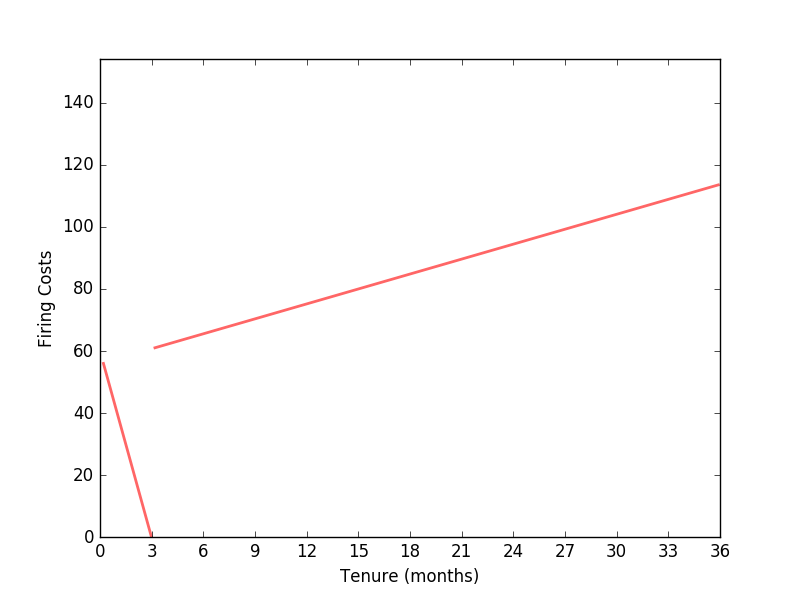
\includegraphics[width=0.8\linewidth]{firingcosts_3months}
  \caption{Firing Cost Schedule (3 Month Probationary Period)}
  \label{fig:firingcosts_3months}
\end{figure}

\newpage

\begin{figure}[h!]
  \centering
  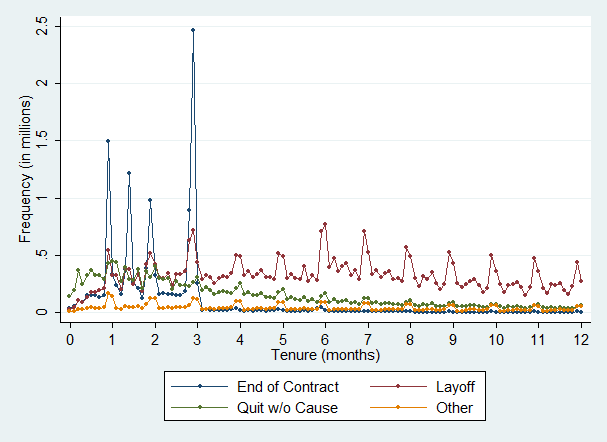
\includegraphics[width=0.8\linewidth]{scatterLL_firings_line}
  \caption{Histogram of Separations by Tenure}
  \label{fig:scatterLL_firings_line}
\end{figure}

\newpage 

\begin{figure}[h!]
  \centering
  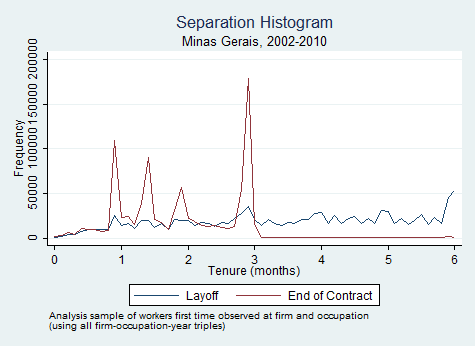
\includegraphics[width=0.8\linewidth]{separationhist_all}
  \caption{Separations for All Firm-Year-Occupations}
  \label{fig:separationhist_all}
\end{figure}

\begin{figure}[h!]
  \centering
  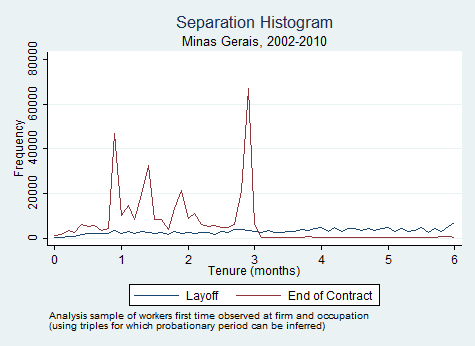
\includegraphics[width=0.8\linewidth]{separationhist_pp}
  \caption{Separations for Restricted Firm-Year-Occupations}
  \label{fig:separationhist_pp}
\end{figure}

\newpage

\begin{figure}[h!]
\begin{subfigure}{.5\textwidth}
  \centering
  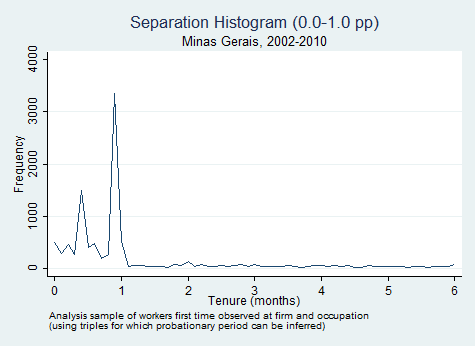
\includegraphics[width=.8\linewidth]{separationhist_pp00-10}
  \caption{1 month}
  \label{fig:separationhist_pp00-10}
\end{subfigure}
\begin{subfigure}{.5\textwidth}
  \centering
  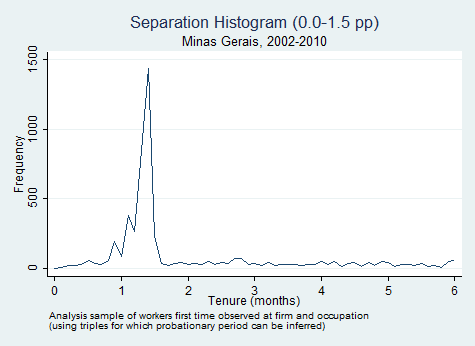
\includegraphics[width=.8\linewidth]{separationhist_pp00-15}
  \caption{1.5 months}
  \label{fig:separationhist_pp00-15}
\end{subfigure}
\begin{subfigure}{.5\textwidth}
  \centering
  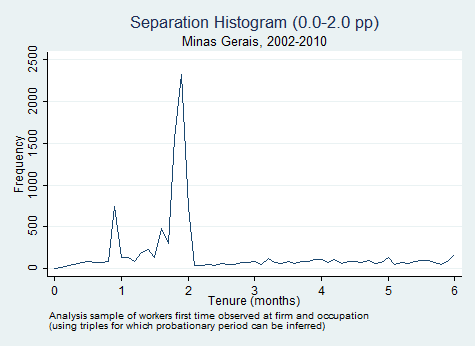
\includegraphics[width=.8\linewidth]{separationhist_pp00-20}
  \caption{2 months}
  \label{fig:separationhist_pp00-20}
\end{subfigure}
\begin{subfigure}{.5\textwidth}
  \centering
  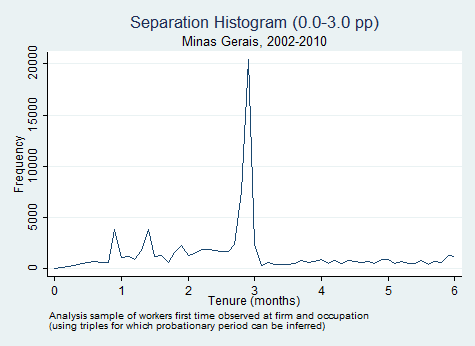
\includegraphics[width=.8\linewidth]{separationhist_pp00-30}
  \caption{3 months}
  \label{fig:separationhist_pp00-30}
\end{subfigure}
\caption{Separation Histograms by Probationary Contracts (without renewal)}
\label{fig:separationhist}
\end{figure}

\newpage 

\begin{figure}[h!]
\begin{subfigure}{.5\textwidth}
  \centering
  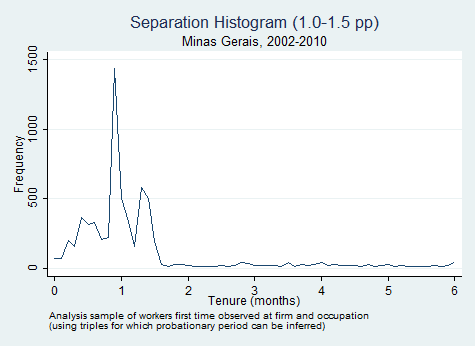
\includegraphics[width=.8\linewidth]{separationhist_pp10-15}
  \caption{1 and 1.5 months}
  \label{fig:separationhist_pp10-15}
\end{subfigure}
\begin{subfigure}{.5\textwidth}
  \centering
  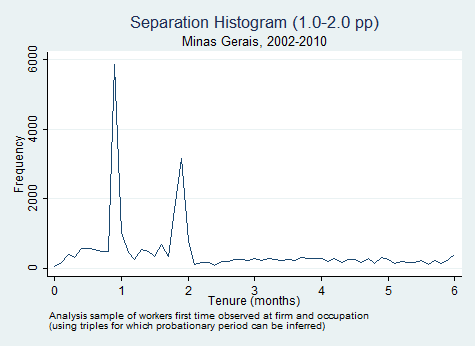
\includegraphics[width=.8\linewidth]{separationhist_pp10-20}
  \caption{1 and 2 months}
  \label{fig:separationhist_pp10-20}
\end{subfigure}
\begin{subfigure}{.5\textwidth}
  \centering
  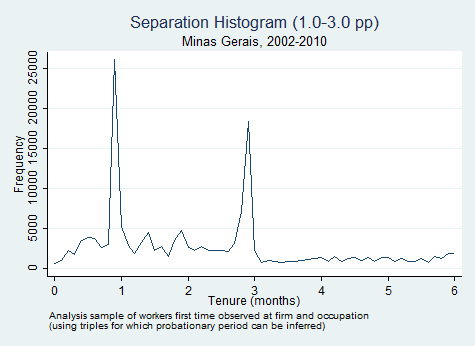
\includegraphics[width=.8\linewidth]{separationhist_pp10-30}
  \caption{1 and 3 months}
  \label{fig:separationhist_pp10-30}
\end{subfigure}
\begin{subfigure}{.5\textwidth}
  \centering
  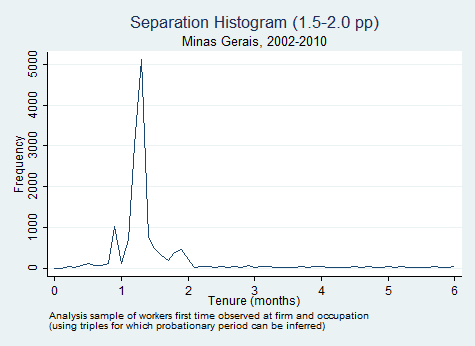
\includegraphics[width=.8\linewidth]{separationhist_pp15-20}
  \caption{1.5 and 2 months}
  \label{fig:separationhist_pp15-20}
\end{subfigure}
\begin{subfigure}{.5\textwidth}
  \centering
  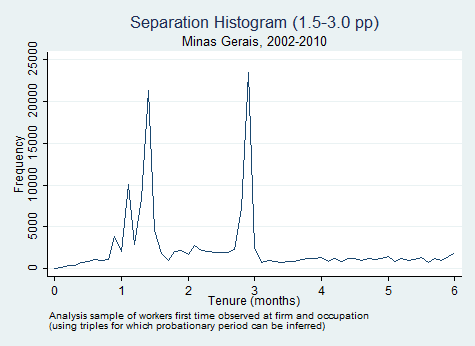
\includegraphics[width=.8\linewidth]{separationhist_pp15-30}
  \caption{1.5 and 3 months}
  \label{fig:separationhist_pp15-30}
\end{subfigure}
\begin{subfigure}{.5\textwidth}
  \centering
  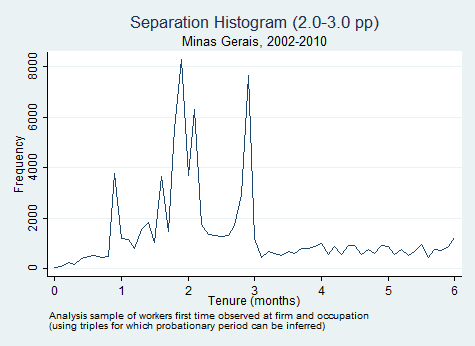
\includegraphics[width=.8\linewidth]{separationhist_pp20-30}
  \caption{2 and 3 months}
  \label{fig:separationhist_pp20-30}
\end{subfigure}
\caption{Separation Histograms by Probationary Contracts (with renewal)}
\label{fig:separationhist_excluded}
\end{figure}

\newpage

\begin{figure}[h!]
  \centering
  \includegraphics[width=0.8\linewidth]{causalgraph_select}
  \caption{Causal Graph (Selection Model)}
  \label{fig:causalgraph_select}
\end{figure}

\begin{itemize}
 \item Histogram of layoffs by tenure (Y): outcome variable
 \item Probationary period length (PP): intervention variable that imposes a discontinuity in firing costs at a particular tenure (within 3 months)
 \item Tenure required for unemployment insurance (UI): at 6 months workers are eligible for unemployment insurance, affecting the histogram of layoffs by tenure
 \item Tenure required for mediation meetings (MM): at 12 months workers that are fired have a mediation meeting, affecting the histogram of layoffs by tenure
 \item Union strength relative to employers (US): the stronger the union is relative to the employer, the shorter the probationary period
 \item Recruitment practices (RP): the shorter the probationary period, the higher the incentive for the employers to improve recruitment practices, thereby affecting the quality of hired employees and monitoring intensity
 \item Quality of applicants (QA): the better the pool of applicants, the higher quality of individuals available for hiring
 \item Quality of hires (QH): the better the hires, the less likely they will be fired during the probationary period
 \item Scope for learning-by-doing (LD): the more room there is for a worker to learn a job with time, the lower the bar set by employers when deciding whether to fire a recent hire, thereby making recruitment practices more important
 \item Monitoring intensity (MI): the shorter the probationary period and the worse the recruitment practices, the more intense the employer will monitor recent hires, thereby affecting the timing of firing decisions by the firm
 \item Location, time, and occupation (S): related to units of observation---can generate backdoor paths (not in Figure~\ref{fig:causalgraph_select} for simplicity)
\end{itemize}

\newpage

\begin{figure}[h!]
  \centering
  \includegraphics[width=0.8\linewidth]{causalgraph_outcome}
  \caption{Causal Graph (Outcome Model)}
  \label{fig:causalgraph_outcome}
\end{figure}

\begin{itemize}
\item Economy-Wide
\begin{itemize}
\item $b$: benefits to be paid on monthly wages
\item $f$: proportion of accumulated wages to be paid as firing fine
\item $\beta$: intertemporal discounting factor
\end{itemize}
\item State-Year-Occupation
\begin{itemize}
\item $k$: probationary contract structure (intervention); determines first and second probationary period cutoffs ($T_k^1$ and $T_k^2$)
\item $y_0$: average match quality in pool of potential workers (net of wages)
\item $\sigma^2_0$: variance of match quality in pool of potential workers
\item $\sigma^2_*$: variance of signals on match quality
\end{itemize}
\item Match-Specific
\begin{itemize}
\item $w$: monthly wage (nominal terms)
\item $h_0$: distribution of match quality in pool of potential workers
$$h_0=\mathcal{N}\left(y_0+\frac{w}{10},\sigma^2_0\right)$$
\item $y_*$: true match quality (also the mean of signals on match quality)
$$y_*\sim \mathcal{N}\left(y_0+\frac{w}{10},\sigma^2_0\right)$$
\item $t_*$: tenure when separation occurs (outcome)
\end{itemize}
\item Evolving by Tenure
\begin{itemize}
\item $\xi$: signal about match quality observed by employer
$$\xi_t\sim\mathcal{N}\left(y_*,\sigma^2_*\right)$$
\item $y$: mean of update to belief on match quality
$$y_t=\left[\frac{(t-1)\sigma^2_0+\sigma^2_*}{t\sigma^2_0+\sigma^2_*}\right]y_{t-1}+\left(\frac{\sigma^2_0}{t\sigma^2_0+\sigma^2_*}\right)\xi_t$$
\item $\sigma^2$: variance of update to belief on match quality
$$\sigma^2_t=\frac{\sigma^2_0\sigma^2_*}{t\sigma^2_0+\sigma^2_*}$$
\item $h$: distribution of match quality beliefs
$$h_t=\mathcal{N}\left(\mu_t,s^2_t\right)$$
where
$$\mu_t=\left(\frac{\sigma^2_0}{t\sigma^2_0+\sigma^2_*}\right)y_*+\left[\frac{(t-1)\sigma^2_0+\sigma^2_*}{t\sigma^2_0+\sigma^2_*}\right]y_{t-1}$$
$$s^2_t=\left(\frac{\sigma^2_0}{t\sigma^2_0+\sigma^2_*}\right)^{1/2}\sigma^2_*$$
\item $R$: revenue generated by match
$$R_t=\xi_t-\frac{w}{10}$$
\item $C$: cost of firing match
\begin{equation} \nonumber
 \begin{split}
  C_t =& \underbrace{\mathbbm{1}\{t\le T_k^1\}[0.5(T_k^1-t)w/10]}_{\text{First Prob. Per.}} \\
& + \underbrace{\mathbbm{1}\{T_k^1 < t\le T_k^2\}[0.5(T_k^2-t)w/10]}_{\text{Second Prob. Per.}} \\
& + \underbrace{\mathbbm{1}\{t> T_k^2\}\left[w\left(1+b+f\left(\frac{t+10}{10}\right)\right)\right]}_{\text{After Prob. Per.}} 
 \end{split}
\end{equation}
\item $d$: firing decision (choice variable)
$$d_t\in\{0,1\}$$
\item $\pi$: profits from current match
$$\pi_t=R_t-\mathbbm{1}\{d_t=1\}C_t$$
\item $V$: value function
$$V_t=\max\{\tilde{V}(d_t=1),\tilde{V}(d_t=0)\}$$
where
$$\tilde{V}(d_t=1)=[R_t-C_t]+\beta\mathbb{E}_{h_0}[V(y',0)]$$
$$\tilde{V}(d_t=0)=[R_t]+\beta\mathbb{E}_{h_t}[V(y',t+1)]$$
so that the firm fires at tenure $t$ (i.e., $d_t=1$) when
$$C_t\le\beta[\mathbb{E}_{h_0}[V(y_{0},0)]-\mathbb{E}_{h_t}[V(y_{t+1},t+1)]]$$
implying that $t_*$ is the lowest $t$ for which $d_t=1$
\end{itemize}
\item Notes
\begin{itemize}
\item The normality assumptions are necessary for applying the Kalman filter
\item The functional form of revenue is irrelevant for the optimal firing decision
\item Assumes workers are fired upon notification and that new match is drawn for the next period (see appendix section \ref{advance_notice})
\item Cost function is constructed from institutional knowledge described in appendix section \ref{firing_costs}
\end{itemize}
\end{itemize}

\newpage

\begin{figure}[h!]
  \centering
  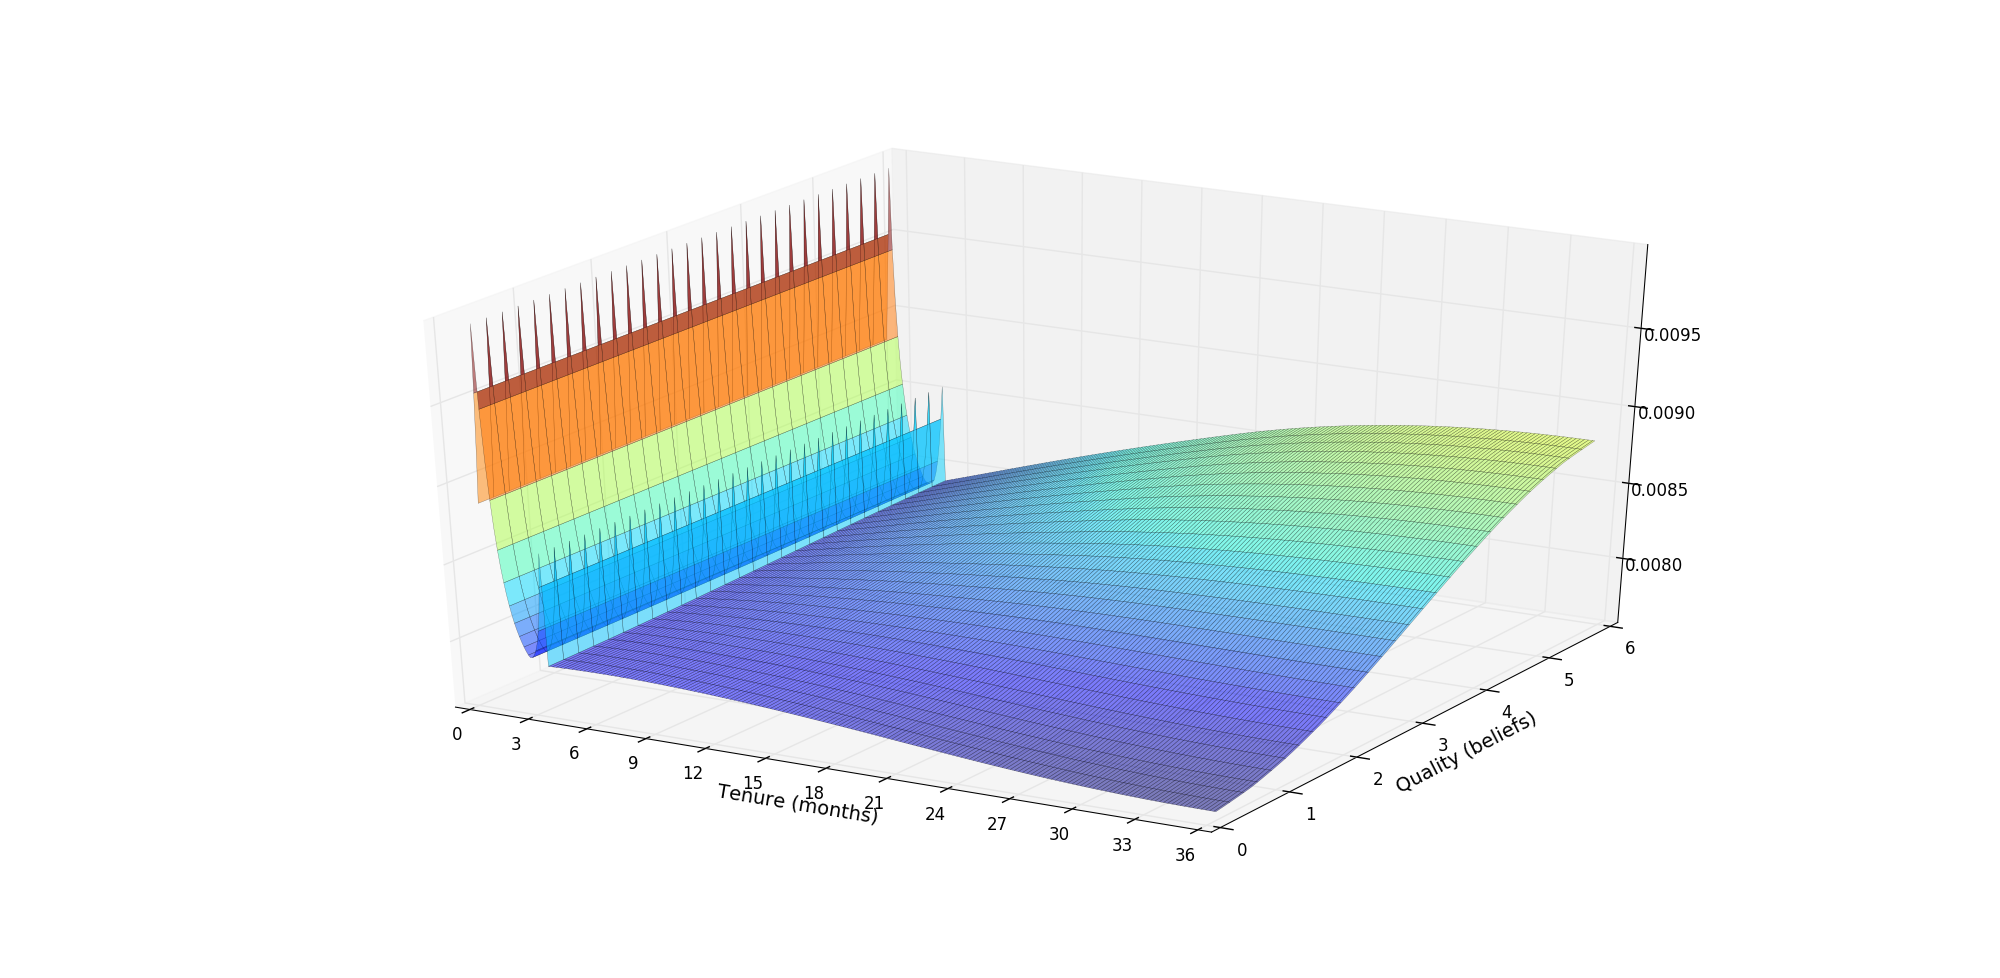
\includegraphics[width=0.8\linewidth]{value_1}
  \caption{Value Function}
  \label{fig:value_1}
\end{figure}

\begin{figure}[h!]
  \centering
  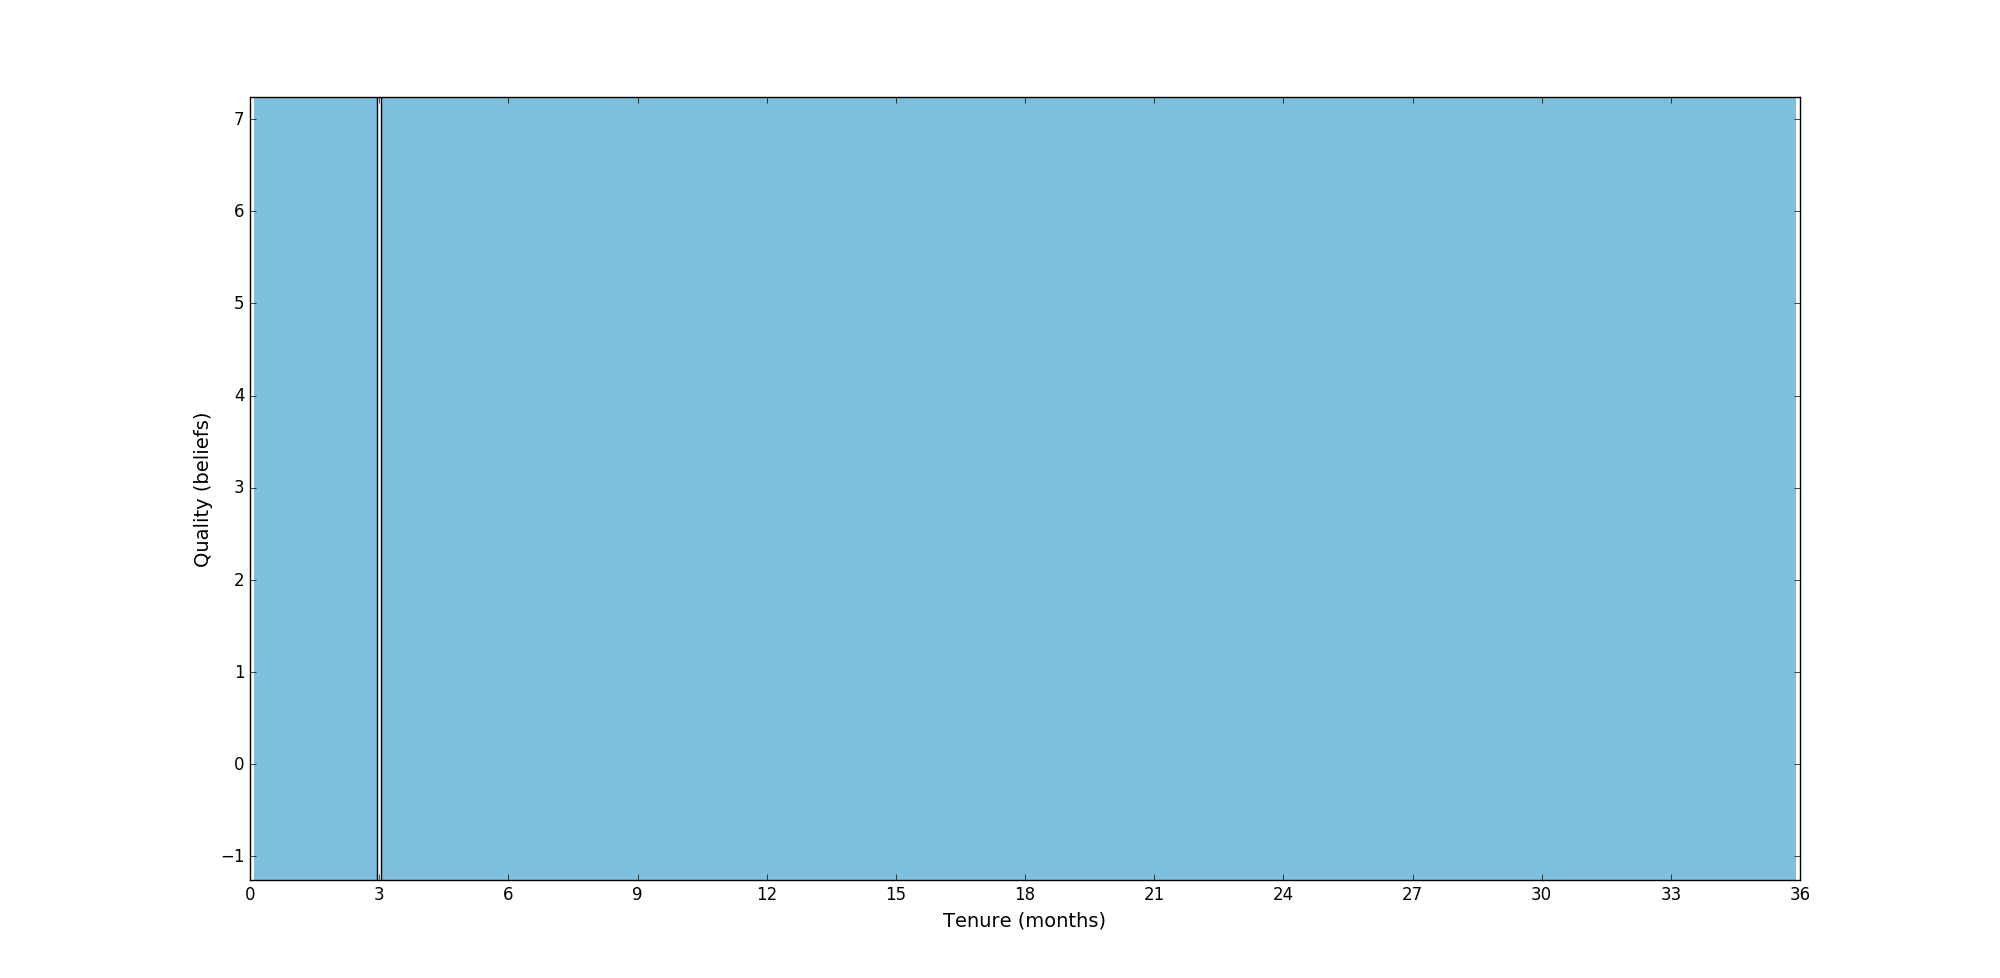
\includegraphics[width=0.8\linewidth]{policy_1}
  \caption{Optimal Policy}
  \label{fig:policy_1}
\end{figure}

\end{document}
